% VUT FIT 3BIT
% ISA 2018/2019
% Project: Programming Network Service
% Author: Vladimir Dusek, xdusek27
% Date: 30/9/2018
% File: isa-assignment.tex

%%%%%%%%%%%%%%%%%%%%%%%%%%%%%%%%%%%%%%%%%%%%%%%%%%%%%%%%%%%%%%%%%%%%%

\documentclass[11pt, a4paper, titlepage]{article}
\usepackage[left=2cm, text={17cm, 24cm}, top=3cm]{geometry}
\usepackage[utf8]{inputenc}
\usepackage[czech]{babel}
\usepackage{pdfpages}
\usepackage[obeyspaces]{url}
\usepackage{framed}
\usepackage[T1]{fontenc}
\usepackage{lmodern}
\usepackage[thinlines]{easytable}
\usepackage{float}

\setlength\parindent{0pt}

%%%%%%%%%%%%%%%%%%%%%%%%%%%%%%%%%%%%%%%%%%%%%%%%%%%%%%%%%%%%%%%%%%%%%

\begin{document}

\begin{titlepage}
	\begin{center}
		\begin{figure}[htb]
			\centering
			
\includegraphics[width=0.85\hsize]{images/fitlogo.pdf}
		\end{figure}
		\vspace{\stretch{0.382}}
		{\Huge Síťové aplikace a správa sítí} \\
		\bigskip
		{\LARGE Dokumentace k~projektu Programování síťové služby} \\
		\bigskip
		{\Large Varianta 2: Export DNS informací pomocí protokolu Syslog}
		\vspace{\stretch{0.618}}
	\end{center}
	{\Large \today \hfill Vladimír Dušek, xdusek27}
\end{titlepage}

%%%%%%%%%%%%%%%%%%%%%%%%%%%%%%%%%%%%%%%%%%%%%%%%%%%%%%%%%%%%%%%%%%%%%

\tableofcontents
\newpage

%%%%%%%%%%%%%%%%%%%%%%%%%%%%%%%%%%%%%%%%%%%%%%%%%%%%%%%%%%%%%%%%%%%%%

\section{Úvod}

Dokumentace popisuje řešení projektu a vysvětluje danou problematiku. Naší úlohou bylo nastudovat si potřebné informace a následně navrhnout, naprogramovat a otestovat síťovou službu, navíc k~ní napsat manuálovou stránku. Varianta 2, kterou jsem řešil spočívala ve vytvoření aplikace dns-export. Ta odposlouchává síťový provoz na síťovém rozhraní, případně zpracovává pcap soubor, ve kterém je nějaká síťová komunikace již zaznamenána. Aplikace vyfiltruje DNS provoz a následně zpracovává jednotlivé pakety, konkrétně DNS odpovědi (responses). V~každé odpovědi projde skrz všechny odpovědní záznamy (Answer resource records) a vyčte určité informace. Doménové jméno, typ DNS záznamu a data specifická pro každý typ. Dále je zaznamenán výskyt těchto informací, shodné jsou sečteny. Tyto výsledky jsou zasílany na syslog server ve formátu odpovídající syslog protokolu.

\newpage

%%%%%%%%%%%%%%%%%%%%%%%%%%%%%%%%%%%%%%%%%%%%%%%%%%%%%%%%%%%%%%%%%%%%%

\section{Uvedení do problematiky}

\subsection{Model TCP/IP}

Síťová komunikace je kvůli své komplexnosti rozdělena do tzv. vrstev, které znázorňují hierarchii činností. Výměna informací mezi vrstvami je přesně definována. Každá vrstva využívá služeb vrstvy nižší a poskytuje své služby vrstvě vyšší.

\subsubsection{Vrstva síťového rozhraní}

Nejnižší vrstva, umožňuje přístup k~fyzickému médiu. Je specifická pro každou síť v~závislosti na její implementaci. (např. Ethernet)

\subsubsection{Síťová vrstva}

Vrstva zajišťuje síťovou adresaci, směrování a předávání datagramů. Je implementována ve všech prvcích sítě -- směrovačích i koncových zařízeních. (např. IPv4, IPv6, ARP, ICMP)

\subsubsection{Transportní vrstva}

Poskytuje transportní služby pro kontrolu celistvosti dat. Jedná se o~spolehlivé spojení (TCP) nebo nespolehlivé spojení (UDP). Je implementována až v~koncových zařízeních, proto umožňuje přizpůsobit chování sítě potřebám aplikace.

\subsubsection{Aplikační vrstva}
Vrstva, která se stará o~přenos konkrétních aplikačních dat. (např. SSH, FTP, HTTP, DHCP, DNS)

\begin{figure}[htp]
    \centering
    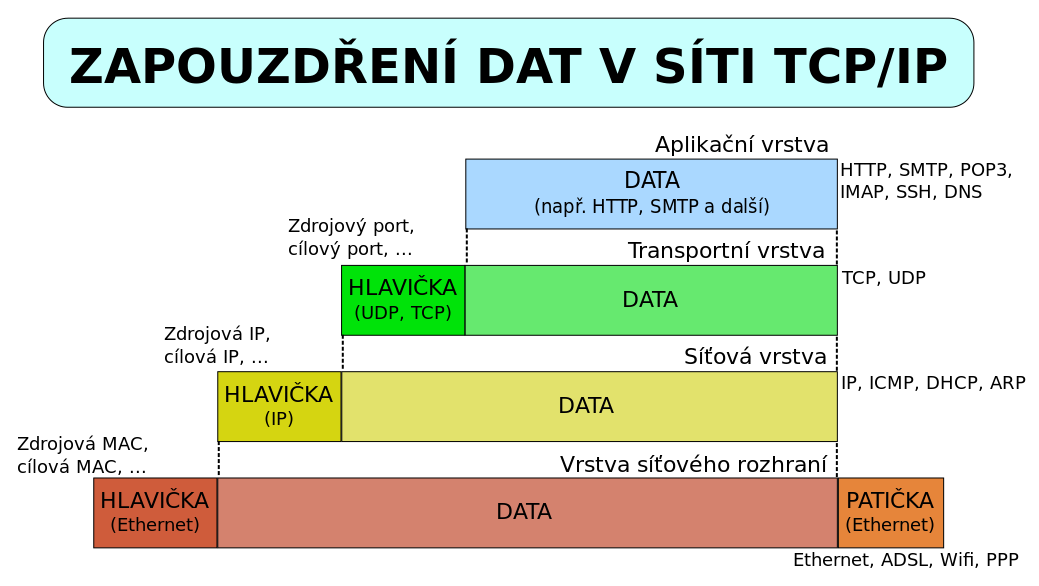
\includegraphics[width=.55\textwidth]{images/layers_schema.png}\hfill
    \caption{Schéma zapouzdření dat na vrstvách TCP/IP}
\end{figure}

\subsection{Domain Name System}

DNS (Domain Name System) je hierarchický systém doménových jmen, který je realizován servery DNS a protokolem stejného jména, kterým si vyměňují informace. Jeho hlavním úkolem jsou vzájemné převody doménových jmen a IP adres sítě. Slouží de facto jako distribuovaná databáze síťových informací.

\subsubsection{Formát DNS zprávy}

DNS zpráva má následující formát:

\begin{table}[H]
	\centering
	\begin{TAB}(r,3cm,0.75cm)[5pt]{|c|}{|c|c|c|c|c|}
		Header \\
		Question \\
		Answer \\
		Authority \\
		Additional \\
	\end{TAB}
\end{table}

Header (hlavička) blíže specifikuje DNS zprávu. Například zda se jedná o~dotaz, či odpověď, zda nastala nějaká chyba, nebo kolik zpráva obsahuje DNS záznamů (resource records) a jakých jsou typů. \\

V~sekci Question (dotaz) jsou informace které chce tázající zjistit. Konkrétně doménové jméno na které se dotazuje, typ a třída záznamu. \\

Answer, Authority a Additional jsou pak záznamy. Všechny mají shodný formát a obsahují různé odpovědi, případně cestu jak se odpovědí dosáhlo.

\subsection{Syslog protokol}

Syslog protokol je standard pro záznam programových zpráv (logů). Program podle protokolu posílá zprávy napříč sítí ke kolektorům logovacích zpráv -- syslog serverům. Jedná se tedy o~architekturu klient-server. Komunikace může probíhat přes UDP na portu 514 nebo přes TCP na portu 6541.

\subsubsection{Formát zpráv}

Maximální délka paketu je 1024 bytů. Zpráva má následující formát:

\begin{center}
	\fbox{PRI HEADER MSG}
\end{center}

Část PRI se skládá ze třech až pěti znaků. Začíná znakem '<', následuje číslo a končí znakem '>'. Číslo uvnitř špičatých závorek se nazývá Priority value a reprezentuje Facility -- zařazení podsystému a Severity -- míru závažnosti.

\begin{center}
	\fbox{PRI = <Priority Value>} \\
\end{center}

Priority value se vypočítá následujícím vzorcem:

\begin{center}
	\fbox{Priority Value = Facility * 8 + Severity}
\end{center}

Část HEADER obsahuje časovou značku -- TIMESTAMP, tedy kdy byla zpráva odeslána a adresu odesílatele -- HOSTNAME, tedy kdo zprávu odeslal.

\begin{center}
	\fbox{HEADER = TIMESTAMP HOSTNAME} \\
\end{center}

Poslední část, MSG, se sestává opět ze dvou částí. První z~nich je TAG, což je název procesu, který zprávu vygeneroval a druhá je CONTENT, tedy konkrétní obsah zprávy.

\begin{center}
	\fbox{MSG = TAG CONTENT} \\
\end{center}

\newpage

%%%%%%%%%%%%%%%%%%%%%%%%%%%%%%%%%%%%%%%%%%%%%%%%%%%%%%%%%%%%%%%%%%%%%

\section{Implementace}

\subsection{Struktura programu}

Aplikace se snaží držet objektově orientovaného paradigma. Kvůli spravování signálů (\path{signal_handler}) bylo nutné některé objekty definovat na globální úrovni.
\bigskip

Jako první se pracuje s~instancí třídy \path{ArgParser}, která se stará o~zpracování argumentů příkazové řádky a jejich validaci. Argumenty jsou uloženy jako privátní atributy a přístup k~nim je definován pomocí příslušných metod.
\bigskip

Třída \path{PcapParser} využívá \path{pcap} knihovnu pro odchytávání síťového provozu na síťovém zařízení, případně pro parsování zdrojového pcap souboru. Dále vyfiltruje DNS provoz a zpracuje veškeré hlavičky až k~aplikační vrstvě. Poradí si na síťové vrstvě s~IPv4 i IPv6 datagramama a na transportní vrstvě s~TCP i UDP komunikací.
\bigskip

Třída \path{DnsParser} zpracovává data DNS protokolu. Vytřídí pouze odpovědi (responses), které neskončili chybou. Projde všechny záznamy v~sekci Answers a vybere data potřebná k~vytvoření statistik. Statistiky ukládá do globální datové struktury \path{unordered_map} jako dvojice klíč->hodnota. Klíč jsou získaná data z~DNS záznamu a value je počet výskytů těchto dat za celou dobu odchytávání, případně za zpracování celého pcap souboru.
\bigskip

Třída \path{Syslog} se pak stará o~komunikaci se syslog serverem. Poskytuje metody pro připojení, odpojení a odesílání zpráv na syslog server.
\bigskip

Ve funkci \path{signal_handler} jsou pak odchytávány signály. \path{SIGUSR1} pro výpis statistik na \path{STDOUT}, \path{SIGALRM} pro odeslání statistik na syslog server a \path{SIGINT} pro ukončení aplikace (v~případě odposlouchávání na síťovém rozhraní běží aplikace až do obdržení tohoto signálu).
\bigskip

V~modulu \path{utils} jsou implementovány pomocné funkce pro zpracovávání DNS komunikace, makro pro debug výpisy, nápověda, či výjimky pro zpracování chybného chování.
\bigskip



\subsection{Popis implementace}

Aplikace je napsaná v~jazyce \path{C/C++} podle standardu \path{C++11}. Překlad je řešen pomocí Unixové utility \path{make} dle přiloženého \path{Makefile} souboru. Dále je napsána manuálová stránka ve značkovacím jazyce \path{troff} -- soubor \path{dns-exp.1}, kde je stručný popis aplikace a jsou blíže specifikovány argumenty a návratové kódy.
\bigskip

Pro zpracování argumentů příkazové řádky je využívána knihovna \path{getopt.h}. Syntaxe zadávání argumentů programu, by tedy měla odpovídat standardním posixovým nástrojům. Například jsou povoleny zkrácené (\path{-a}) i dlouhé (\path{--argument}) varianty argumentů a jejich libovolné pořadí.
\bigskip

Pro zachytávání provozu na síťovém rozhraní, či zpracovávání pcap souboru aplikace využívá funkce \path{pcap} knihovny. Ta také komunikaci vyfiltruje pouze na DNS komunikaci. Funkce \path{pcap_loop} iteruje přes veškeré vyfiltrované rámce. Každý z~nich je zpracováván ve statické metodě \path{packet_handle}. Zde je zpracování dále děleno. Nejprve na vrtsvě síťového rozhraní (network interface layer) podle typu rámce -- Ethernet, SSL. Poté na síťové vrstvě (network layer) podle typu datagramu -- \path{IPv4}, \path{IPv6}. Nakonec i podle typu packetu na vrstvě transportní (transport layer) -- \path{TCP}, \path{UDP}. Při \path{UDP} komunikaci je řízení rovnou předáváno modulu DnsParser. V~případě TCP komunikaci, jsou data ukládána do globálního bufferu (\path{vector}) a zpracována až v~případě nutnosti -- před odesláním na syslog server, či vypsáním na \path{STDOUT}. Je tomu tak z~důvodu fragmentace aplikačních dat DNS na transportní vrstvě.
\bigskip

Modul \path{DnsParser} pak sbírá už konkrétní informace. Tedy na jaké doménové jméno byl kladen dotaz, jaký typ dotazu byl požadován a konkrétní odpověď. Jsou podporovány následující DNS typy: A, AAAA, CNAME, DNSKEY, DS, MX, NS, NSEC, OPT, PTR, RRSIG, SOA, SPF a TXT. Ostaní typy jsou značeny jako \path{unknown_type} a jejich data jako \path{unknown_data}. Pro přehlednost výpisu je u~položek Digest (DS), Public key (DNSKEY) a Signature (RRSIG) vypsáno pouze 20 prvních znaků následováno třemi tečkami. Modul využívá různých implementovaných struktur pro ulehčení práce s~ukazateli. U~struktur je použit atribut \path{__attribute__((packed))}, aby nedocházelo k~jejich zarovnání (padding).
\bigskip

Komunikace se syslog serverem je řešeno pomocí knihovny \path{sys/socket.h}. Nejprve je navázáno komunikace se serverem a poté jsou zprávy (logs) postupně odesílány. Před skončením aplikace je spojení ukončeno a socket uzavřen.
\bigskip



\subsection{Návratové kódy}

\begin{itemize}
	\item 0 -- OK
	\item 1 -- chyba zpracování argumentů příkazové řádky
	\item 2 -- chyba při odposlouchávání síťového rozhraní či zpracování pcap souboru (např. neplatné jméno rozhraní nebo pcap souboru)
	\item 3 -- chyba při komunikaci se syslog serverem (např. nepodařilo se navázat spojení)
	\item 9 -- systémová chyba (např. malloc nealokoval paměť)
\end{itemize}

\newpage

%%%%%%%%%%%%%%%%%%%%%%%%%%%%%%%%%%%%%%%%%%%%%%%%%%%%%%%%%%%%%%%%%%%%%

% \section{Testování}

% ...

% \newpage

%%%%%%%%%%%%%%%%%%%%%%%%%%%%%%%%%%%%%%%%%%%%%%%%%%%%%%%%%%%%%%%%%%%%%

\section{Použití}

\subsection{Překlad}

\begin{description}
	\item \path{$ make} -- pro standardní překlad programu
	\item \path{$ make pack} -- pro překlad programu pro účely debugování (přepínač \path{-g}, debugovací vypisy)
	\item \path{$ make clean} -- pro smazání všech objektových souborů a deplistu
	\item \path{$ make clean-all} -- pro smazání všech objektových souborů, deplistu a binárního souboru
\end{description}
\smallskip



\subsection{Spuštění}

\path{$ ./dns-export [-r RESOURCE | -i INTERFACE] [-t TIMEOUT] [-s SERVER] [-h]}

\begin{itemize}
	\item \path{-r RESOURCE}, \path{--resource RESOURCE} -- Udává jméno pcap souboru, který se bude zpracovávát. Aspoň jeden z~argumentů \path{resource} nebo \path{interface} musí být zadán.

	\item \path{-i INTERFACE}, \path{--interface INTERFACE} -- Udává jméno rozhraní na kterém bude odposloucháván síťový provoz. Aspoň jeden z~argumentů \path{resource} nebo \path{interface} musí být zadán.

	\item \path{-t TIMEOUT}, \path{--timeout TIMEOUT} -- Časový interval v~sekundách udávající, jak často statistiky budou zasílány. Výchozí hodnota 60 vteřin. Volitelný argument.

	\item \path{-s SERVER}, \path{--server SERVER} -- Adresa syslog serveru kam statistiky budou zasílány. Výchozí adresa je localhost. Volitelný argument.

	\item \path{-h}, \path{--help} -- Vypíše nápovědu na \path{STDOUT}. Volitelný argument.
\end{itemize}
\smallskip



\subsection{Příklady spuštění}

\subsubsection{Zpracovávání pcap souboru}

Spuštění aplikace pro zpracování \path{dns.pcap} souboru a odesílání zpráv (logs) na lokální syslog server.

\begin{center}
    \fbox{\path{$ ./dns-export -r dns.pcap -s localhost}}
\end{center}

Po ukončení běhu aplikace si můžeme zobrazit výsledné zprávý. Ty jsou uloženy podle konfigurace syslogu. Výchozí cesta je \path{/var/log/messages}. Pro jejich zobrazení můžeme použít například nástroj \path{journalctl}, který slouží pro zobrazení systémových zpráv. Ten obsahuje řadu přepínačů pro vyfiltrování konkrétnějšího obsahu. Pokud máme dostupná práva \path{root}, můžeme si soubor přímo vypsat. Například utilita \path{tail} nám vypíše posledních n řádků souboru.

\begin{center}
    \fbox{\path{# tail -n 5 /var/log/messages}}
\end{center}

\scriptsize

\path{<134>1 2018-10-26T13:57:28.703Z 192.168.122.1 dns-export --- www.youtube.com CNAME youtube-ui.l.google.com 1}

\path{<134>1 2018-10-26T13:57:28.703Z 192.168.122.1 dns-export --- widgets.getsitecontrol.com CNAME gscwidgets.b-cdn.net 1}

\path{<134>1 2018-10-26T13:57:28.703Z 192.168.122.1 dns-export --- youtube-ui.l.google.com A~172.217.23.238 1}

\path{<134>1 2018-10-26T13:57:28.703Z 192.168.122.1 dns-export --- www.yahoo.com CNAME atsv2-fp-shed.wg1.b.yahoo.com 1}

\path{<134>1 2018-10-26T13:57:28.703Z 192.168.122.1 dns-export --- photos-ugc.l.googleusercontent.com A~172.217.23.225 1}

\normalsize

\subsubsection{Odposlouchávání na síťovém rozhraní}

Spuštění aplikace pro odposloucháváné provozu na síťovém rozhraní \path{eth0}. Jsou vyžadována práva \path{root}.

\begin{center}
    \fbox{\path{# ./dns-export -i eth0 -s localhost -t 30}}
\end{center}

Při obdržení signálu \path{SIGUSR1} nám aplikace vypíše na \path{STDOUT} dosud nasbírané statistiky. Jelikož zasílámě signál aplikaci která běží s~právama \path{root}, potřebujeme je i při zaslání signálu. Abychom mohli zaslat procesu signál, potřebujeme znát jeho ID. To zjistíme například:

\begin{center}
    \fbox{\path{$ ps aux | grep dns-export}}
\end{center}

\scriptsize

\path{root      6445  0.0  0.1 372536  9484 pts/1    S+   13:05   0:00 sudo ./dns-export -i eth0 -s localhost -t 30}

\normalsize

\medskip

Zaslání signálu pak vypadá následovně:

\begin{center}
    \fbox{\path{# kill -SIGUSR1 6445}}
\end{center}

\scriptsize

\path{i.stack.imgur.com.cdn.cloudflare.net A~104.16.30.34 1}

\path{i.stack.imgur.com CNAME i.stack.imgur.com.cdn.cloudflare.net 1}

\path{cdn.sstatic.net A~151.101.193.69 1}

\path{stackoverflow.com A~151.101.1.69 1}

\path{cdn.sstatic.net A~151.101.1.69 1}

\normalsize

\medskip

Aplikace běží až do obdržení signálu \path{SIGINT}, ten lze zaslat aplikaci klávesami \path{CTRL+C}. Ještě před skončením jsou zaslány sesbírané statistiky na syslog server. Zobrazit si je můžeme stejně jako v~případě se zpracováním pcap souboru.

\newpage

%%%%%%%%%%%%%%%%%%%%%%%%%%%%%%%%%%%%%%%%%%%%%%%%%%%%%%%%%%%%%%%%%%%%%

\section{Závěr}

Celý projekt se skládá z~následujících zdrojových souborů \path{C++}: \path{main.cpp}, \path{arg_parser.cpp}, \path{arg_parser.h}, \path{pcap_parser.cpp}, \path{pcap_parser.h}, \path{dns_parser.cpp}, \path{dns_parser.h}, \path{syslog.cpp}, \path{syslog.h}, \path{utils.cpp}, \path{utils.h} a souboru pro překlad \path{Makefile}. To je celkem 2279 řádků kódu. Velikost výsledného binárního souboru \path{dns-export} je 161.2\,KiB. Dále dokumentace v~sázecím systému \path{LaTeX}: \path{manual.pdf} a manuálové stránky ve značkovacím jazyce \path{troff}: \path{dns-export.1}.
\bigskip

Práce na projektu byla bez pochyby velmi zajímavá a přínosná. Zdokonalil jsem se ve psaní v~C++, poznal pcap knihovnu, na vlastní kůži viděl jak funguje TCP/IP zásobník, poměrně do detailů si nastudoval DNS, vyzkoušel si komunikaci se syslogem a napsal manuálovou stránku. Na druhou stranu musím zmínit, že časová náročnost projektu velmi přesahovala deklarovanu časovou zátěž v~kartě předmětu. K~čemu tu pak máme kreditový systém ECTS s~cílem sjednocovat studijní zátěž vysokoškolského studia napříč EU. Takto přestřelená časová zátěž je pak pouze na úkor docházky na přednáškách, práce na projektech do jiných předmětů, či, nyní ve třetím ročníku, na bakalářské práci.

\newpage

%%%%%%%%%%%%%%%%%%%%%%%%%%%%%%%%%%%%%%%%%%%%%%%%%%%%%%%%%%%%%%%%%%%%%

\renewcommand{\refname}{Zdroje}
\addcontentsline{toc}{section}{Zdroje}
\begin{thebibliography}{9}
\bibitem{bl}
    IANA,
    Domain Name System Security (DNSSEC) Algorithm Numbers [online],
    2017-03-10,
    \url{https://www.iana.org/assignments/dns-sec-alg-numbers/dns-sec-alg-numbers.xhtml},
    [cit. 2018-10-27]
\bibitem{bl}
    IANA,
    Delegation Signer (DS) Resource Record (RR) Type Digest Algorithms [online],
    2012-04-13,
    \url{https://www.iana.org/assignments/ds-rr-types/ds-rr-types.xhtml},
    [cit. 2018-10-27]
\bibitem{bl}
    IANA,
    Domain Name System (DNS) Parameters [online],
    2018-09-17,
    \url{https://www.iana.org/assignments/dns-parameters/dns-parameters.xhtml},
    [cit. 2018-10-27]
\bibitem{bl}
    Network Working Group,
    RFC 1035 - Domain names - implementation and specification [online],
    1987-11,
    \url{https://tools.ietf.org/html/rfc1035},
    [cit. 2018-10-27]
\bibitem{bl}
    Network Working Group,
    RFC 3164 - The BSD syslog Protocol [online],
    2001-08,
    \url{https://tools.ietf.org/html/rfc3164},
    [cit. 2018-10-27]
\bibitem{bl}
    Network Working Group,
    RFC 3339 - Date and Time on the Internet: Timestamps [online],
    2002-07,
    \url{https://tools.ietf.org/html/rfc3339},
    [cit. 2018-10-27]
\bibitem{bl}
    Network Working Group,
    RFC 3596 - DNS Extensions to Support IP Version 6 [online],
    2003-10,
    \url{https://tools.ietf.org/html/rfc3596},
    [cit. 2018-10-27]
\bibitem{bl}
    Network Working Group,
    RFC 4034 - Resource Records for the DNS Security Extensions [online],
    2005-03,
    \url{https://tools.ietf.org/html/rfc4034},
    [cit. 2018-10-27]
\bibitem{bl}
    Network Working Group,
    RFC 5424 - The Syslog Protocol [online],
    2009-03,
    \url{https://tools.ietf.org/html/rfc5424},
    [cit. 2018-10-27]
\bibitem{bl}
    Wikipedia contributors,
    Domain Name System [online],
    2018-10-26,
    \url{https://en.wikipedia.org/wiki/Domain_Name_System/},
    [cit. 2018-10-27]
\bibitem{bl}
    Wikipedia contributors,
    List of DNS record types [online],
    2018-10-18,
    \url{https://en.wikipedia.org/wiki/List_of_DNS_record_types/},
    [cit. 2018-10-27]
\bibitem{bl}
    Wikipedia contributors,
    Domain Name System Security Extensions [online],
    2018-10-05,
    \url{https://en.wikipedia.org/wiki/Domain_Name_System_Security_Extensions},
    [cit. 2018-10-27]
\bibitem{bl}
    Redhat,
    How to configure remote logging with rsyslog [online],
    2018-08-29,
    \url{https://access.redhat.com/solutions/54363},
    [cit. 2018-10-27]
\bibitem{bl}
    Keyboard Banger,
    DNS Message Format And Name Compression [online],
    2015-09-25,
    \url{http://www.keyboardbanger.com/dns-message-format-name-compression/},
    [cit. 2018-10-27]
\bibitem{bl}
    firewall.cx,
    DNS QUERY MESSAGE FORMAT [online],
    2012,
    \url{http://www.firewall.cx/networking-topics/protocols/domain-name-system-dns/160-protocols-dns-query.html},
    [cit. 2018-10-27]
\bibitem{bl}
    Michael Kerrisk, man7.org,
    linux/man-pages [online],
    2018-10,
    \url{http://man7.org/linux/man-pages/man3/},
    [cit. 2018-10-27]
\bibitem{bl}
    Lars Wirzenius,
    Writing manual pages [online],
    2018-07,
    \url{https://liw.fi/manpages/},
    [cit. 2018-10-27]
\bibitem{bl}
    The Tcpdump team,
    Pcap library manual page [online],
    2018-10,
    \url{https://www.tcpdump.org/manpages/},
    [cit. 2018-10-27]
\end{thebibliography}

%%%%%%%%%%%%%%%%%%%%%%%%%%%%%%%%%%%%%%%%%%%%%%%%%%%%%%%%%%%%%%%%%%%%%

\end{document}
